\section{UI Animations}
\label{sec:ui_animations}

This paper develops a DSL for creating GUI animations. This section gives a high-level overview of the problem domain and the expected features of the DSL.

\subsection{Problem Domain}

Graphical user interfaces typically use various concepts to aid users in understanding what the application is doing. One example is to display brief animations whenever the interface changes shape.

For example, in Figure~\ref{fig:usecase1} a menu is displayed on the screen when the corresponding icon is pressed. This menu slides in from the right while the background fades out.

\begin{figure}[H]
\centering
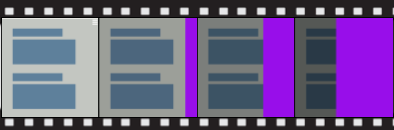
\includegraphics[scale=0.4]{pictures/usecase1fig.png}
\caption{Animation of a menu sliding in from the right while the background fades out.}
\label{fig:usecase1}
\end{figure}

Another example can be seen in Figure~\ref{fig:usecase2}, where a user can click on a location to move the character in the game. The application displays an animation to indicate the button press is received correctly and then the character moves to the selected location.

\begin{figure}[H]
\centering

\includegraphics[scale=0.4]{pictures/todo.png}
\caption{An animation is played to indicate the selected location, then the character moves to this location.}
\label{fig:usecase2}
\end{figure}

\subsection{Composing Animations}

The DSL expresses animations by composing smaller parts together. A \emph{basic} animation expresses an elementary unit of animation, which is typically one varying property within the interface. On the other hand, \emph{composed} animations creates a bigger animation out of smaller animations.

\subsubsection{Basic Animations}

A basic animation changes the value of an element in the UI over a period of time. To specify a basic animation we need three elements. First, a lens specifies which property in our UI should change. Second, we provide the target value for this property. Third, we provide the duration, specifying how many seconds the animation should last.

In the menu use case of Figure~\ref{fig:usecase1} there are two properties which need to change during the animation: the x-value of the incoming menu and the alpha property of the box obscuring the application. We express this using the \hs{basic} operation.

First we need to create the animation which makes the menu slide in. We pass three parameters to the \hs{basic} operation: the lens \hs{menu . x} which focuses on the x-value of the incoming menu, the duration \hs{For 0.5} and the target value \hs{To 25}. This results in the animation seen in Figure~\ref{fig:usecase1basic1}.

\begin{code}
menuSlideIn = basic (menu . x) (For 0.5) (To 25)
\end{code}

\begin{figure}[H]
\centering

\includegraphics[scale=0.4]{pictures/usecase1basic1.png}
\caption{...}
\label{fig:usecase1basic1}
\end{figure}

Second we also need to create an animation which fades out the application. Now the lens focuses on the alpha-value of the obscuring box and sets it to \hs{0.6} over \hs{0.5} seconds. This results in the animation seen in Figure~\ref{fig:usecase1basic2}.

\begin{code}
appFadeOut = basic (obscuringBox . alpha) (For 0.5) (To 0.6)
\end{code}

\begin{figure}[H]
\centering
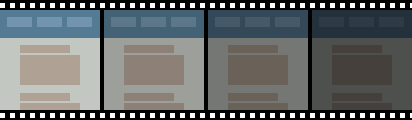
\includegraphics[scale=0.4]{pictures/usecase1basic2.png}
\caption{...}
\label{fig:usecase1basic2}
\end{figure}

\subsubsection{Composed Animations}

A composed animation combines several other animations into one new animation. We can do this either in \emph{sequence} or in \emph{parallel}.

For the menu use case we want to display the animations \hs{menuSlideIn} and \hs{appFadeOut} at the same time. Thus, we create a composed animation using \hs{par},  which results in the animation as seen in Figure~\ref{fig:usecase1}.

\begin{code}
menuAnimation = menuSlideIn `par` appFadeOut
\end{code}

For the game use case we want to display the animations \hs{selectedIndicator} and \hs{playerMove} one after the other. To do this we create a composed animation using \hs{seq}, which results in the animation as seen in Figure~\ref{fig:usecase2}.

\subsection{Additional Requirements}

In addition to the previous features, we also expect the DSL to support two additional requirements: the user can embed custom operations and inspect an animation specified with the DSL.

\subsubsection{Custom Operations}

% Other UI Animation Libraries:
% https://www.codementor.io/hayeskier/7-best-animation-libraries-for-ui-designers-2018-kmg7byy1g
% https://greensock.com/docs/
% https://animejs.com/documentation/#cssSelector

The DSL also supports embedding of any arbitrary effect. For example we can embed an \hs{IO} operation, playing a sound effect, in the middle of a sequence of animations.
\begin{code}
upThenBeepThenRight = seq [moveUp, beep, moveRight]
\end{code}


\subsubsection{Inspection}


\subsection{Examples}

